\documentclass[conference]{IEEEtran}
\usepackage{amsmath}
\usepackage{graphicx}
\usepackage{url}
\usepackage[hidelinks]{hyperref}

\begin{document}

\title{CloudNative Job Finder: A Cloud-Native Distributed Job Search Platform}

\author{
\IEEEauthorblockN{Shardendu Mishra}
\IEEEauthorblockA{
23BCS122 \\
23bcs122@iiitdwd.ac.in
}
\and
\IEEEauthorblockN{Anas Khan}
\IEEEauthorblockA{
23BCS083 \\
23bcs083@iiitdwd.ac.in
}
\and
\IEEEauthorblockN{Mayank Bansal}
\IEEEauthorblockA{
23BEC026 \\
23bec026@iiitdwd.ac.in
}
}

\maketitle

\begin{abstract}
Cloud-Native Job Finder is a cloud-native distributed platform for resume-aware job discovery under continuously changing external data. The system is implemented using microservices in Go and Python, a Next.js frontend, asynchronous event processing, and containerized infrastructure.
The architecture separates user-facing REST APIs from long-running ingestion and ranking workers, enabling independent scaling and failure isolation. Transactional data is stored in PostgreSQL, resume binaries in MinIO, recommendation responses in Redis, and searchable job documents in Meilisearch.
Event propagation is handled through an outbox relay with RabbitMQ and Kafka support, enabling retry-aware delivery and staged stream evolution.
This report presents a repository-grounded analysis of system structure, communication pipeline, technology rationale, deployment model, and engineering trade-offs.
\href{https://github.com/Team-Parashuram/CloudNative-Job-Finder}{GitHub Link - Repository}
\end{abstract}

\begin{IEEEkeywords} 
cloud-native systems, microservices, event-driven architecture, distributed recommendation, outbox pattern
\end{IEEEkeywords}

\section{Introduction}
Job search systems must process high-churn external listings, parse unstructured resumes, compute personalized relevance, and expose low-latency user APIs. These concerns have heterogeneous performance profiles: authentication and profile reads are latency-sensitive, while scraping and parsing are bursty and failure-prone. A single monolith ties these workloads together and amplifies tail latency during ingestion spikes.

CloudNative Job Finder addresses this through service decomposition and asynchronous pipelines. The repository organizes API ingress, identity, resume ingestion, scraping, enrichment, matching, recommendation serving, scheduling, outbox relay, and behavioral feature aggregation as independently deployable services. The design target is not only feature coverage, but operational robustness under partial failure and evolving transport layers.

\section{System Architecture}
\subsection{Architecture Overview}
The end-to-end path is: frontend $\rightarrow$ API gateway $\rightarrow$ internal services $\rightarrow$ event broker/stream $\rightarrow$ worker services $\rightarrow$ storage/indexing $\rightarrow$ recommendation APIs. Synchronous REST is used where immediate user response is required; asynchronous events are used where processing is long-running or fan-out oriented.

\begin{figure}[h]
\centering
\IfFileExists{architecture.png}{
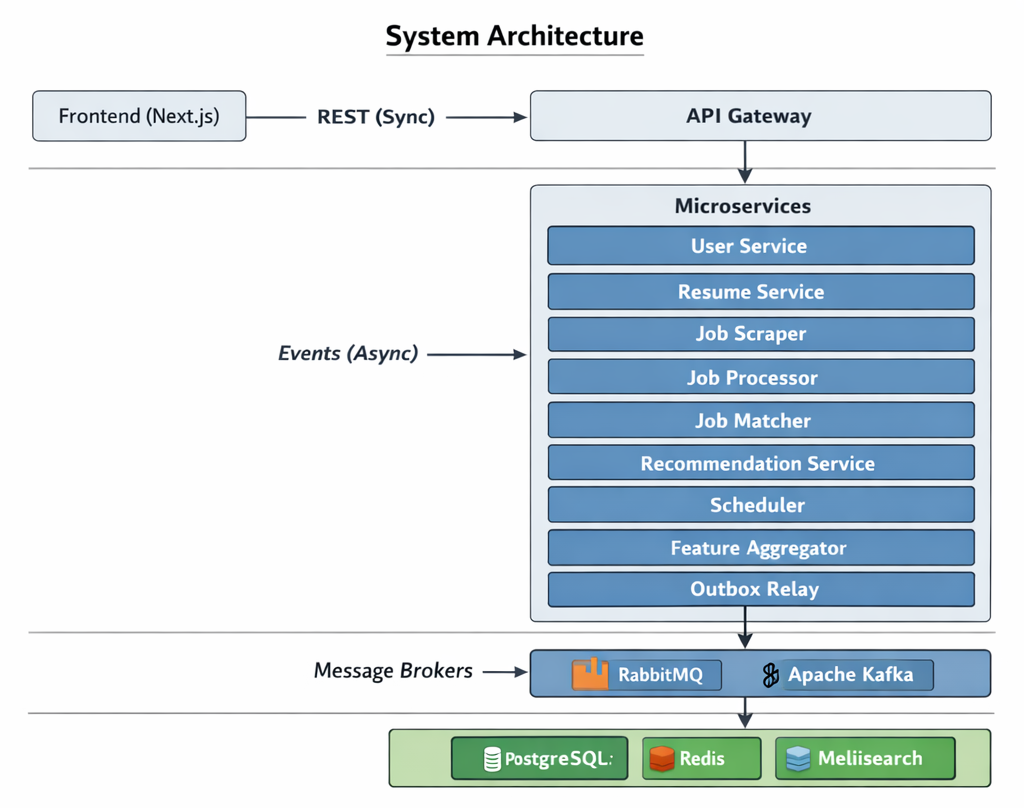
\includegraphics[width=0.45\textwidth]{architecture.png}
}{
\fbox{\parbox[c][0.11\textheight][c]{0.42\textwidth}{\centering architecture.png unavailable.\\System Architecture placeholder.}}
}
\caption{System Architecture}
\label{fig:architecture}
\end{figure}

\subsection{Microservices and Event-Driven Justification}
The architecture is explicitly microservices-based and event-driven. Microservices are used for scalability and fault isolation: scraper/parser faults do not directly impact login or recommendation reads. Event-driven processing provides decoupling and throughput smoothing: producers publish lifecycle facts, and consumers process independently with retries and restart tolerance. Independent deployment follows naturally because service contracts are HTTP endpoints plus stable event payload schemas.

\section{Component Breakdown}
\subsection{Frontend}
The frontend is a Next.js App Router application with protected routes (dashboard, resumes, recommendations, profile), cookie-backed JWT handling, and API rewrite/proxy behavior through the gateway. This exists to centralize public API exposure and avoid direct browser coupling to internal service topology.

\subsection{Services}
\textbf{api-gateway} handles JWT issuance/validation, request proxying, and interaction event publication; \textbf{user-service} isolates credential hashing and profile state; \textbf{resume-service} owns resume metadata/object keys and parsed keyword updates; \textbf{resume-parser} consumes \texttt{resume\_uploaded}, parses documents, and calls internal parsed-update endpoints; \textbf{job-scraper} concurrently ingests RemoteOK, WeWorkRemotely, and Hacker News with fingerprint deduplication; \textbf{job-processor} cleans text, extracts keywords, updates jobs, and indexes Meilisearch; \textbf{job-matcher} computes hybrid ranking and writes \texttt{resume\_job\_matches}; \textbf{recommendation-service} serves paginated read models with Redis caching; \textbf{scheduler} drives cron-based scrape/match/email automation; \textbf{outbox-relay} publishes pending outbox records to Kafka and optionally mirrors RabbitMQ; \textbf{feature-aggregator} updates user-job behavioral features from interaction streams.

Each service exists to isolate a distinct failure domain and scaling axis. This avoids over-coupling ingestion throughput to user-facing latency.

\subsection{Shared and Infrastructure Layers}
The \texttt{shared/} layer provides event contracts, queue/stream clients, BM25 scoring, idempotency, workflow-state transitions, telemetry middleware, and utility modules. Infrastructure via Docker Compose provisions PostgreSQL, Redis, RabbitMQ, Kafka/Zookeeper, MinIO, Meilisearch, and all services with health checks and dependency ordering.

\section{Communication and Data Flow}
\subsection{Pipeline: Scraping to Recommendation}
The implemented producer-consumer flow is:
\begin{enumerate}
\item Resume upload: gateway forwards file; resume-service stores MinIO object + DB row and enqueues \texttt{resume\_uploaded} through outbox.
\item Parsing: resume-parser consumes event, extracts skills/keywords/job-title hints, and updates resume-service; resume-service emits \texttt{resume\_parsed}.
\item Job ingestion: scheduler triggers scraper; scraper upserts normalized jobs and enqueues \texttt{job\_scraped}; processor consumes, enriches, indexes Meilisearch, emits \texttt{job\_indexed}.
\item Matching and serving: matcher consumes readiness events, writes ranked matches, emits \texttt{job\_matches\_generated}; recommendation-service serves cached paginated recommendations; scheduler sends immediate and weekly email notifications.
\end{enumerate}

\begin{figure}[h]
\centering
\IfFileExists{dataflow.png}{
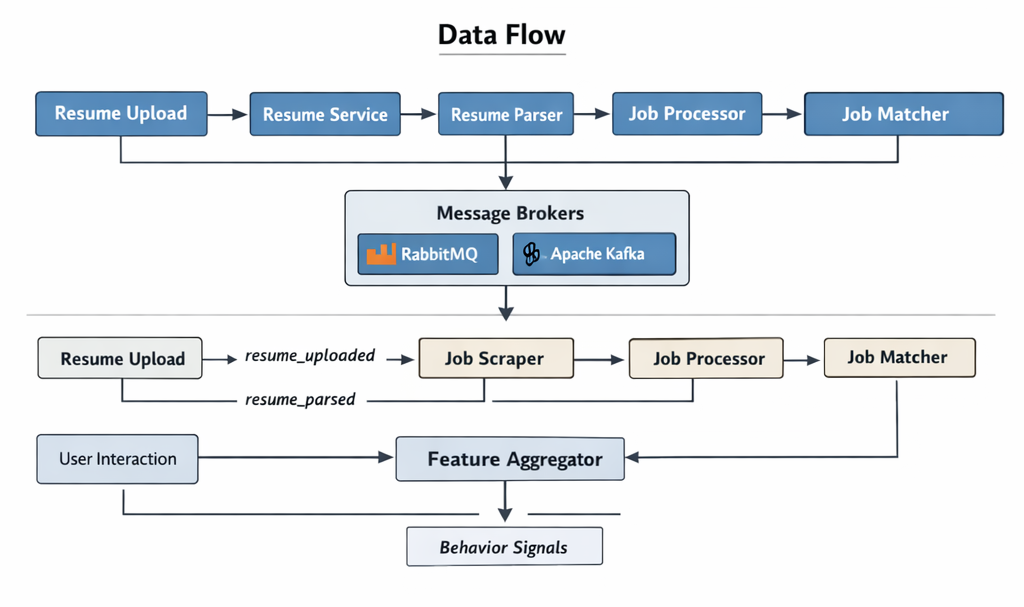
\includegraphics[width=0.45\textwidth]{dataflow.png}
}{
\fbox{\parbox[c][0.11\textheight][c]{0.42\textwidth}{\centering dataflow.png unavailable.\\Data Flow placeholder.}}
}
\caption{Data Flow}
\label{fig:dataflow}
\end{figure}

\subsection{Asynchrony and Reliability}
RabbitMQ consumers use explicit ack/nack behavior; Kafka consumers use group commits plus event-id deduplication via \texttt{processed\_events}. The outbox pattern decouples transactional writes from broker publication, with retry counts, failure states, and dead-letter routing support. This design is selected to reduce dual-write inconsistency and duplicate side effects during retries or restarts.

\section{Technologies Used}
\subsection{Language and Runtime Choices}
Go is used for most services because it provides efficient concurrency and simple operational binaries; goroutines are used in concurrent scraping and long-running consumers. Python is used for resume parsing due to stronger document/NLP tooling (PyMuPDF, pdfminer, NLTK, spaCy), making extraction quality easier to iterate without destabilizing the rest of the stack.

\subsection{Messaging, Data, and Search Stack}
RabbitMQ provides routing-key event distribution for domain transitions; Kafka provides versioned stream topics and consumer-group processing. PostgreSQL stores users, resumes, jobs, matches, outbox rows, idempotency state, behavioral features, and pipeline states. Redis reduces recommendation read latency via short-lived page caching. MinIO separates binary object storage from relational metadata. Meilisearch supports low-latency indexed retrieval and filtering for enriched job records.

\subsection{Scheduling, APIs, and Scoring}
The scheduler uses cron expressions for scrape, match-all, and weekly email tasks, plus startup bootstrap to reduce cold-start recommendation gaps. Inter-service synchronous calls are REST with internal token headers; gRPC is currently reserved as future work via a proto placeholder. Ranking is hybridized in code:
\begin{equation}
S = 100\left(0.45S_{\mathrm{bm25}} + 0.20S_{\mathrm{sem}} + 0.25S_{\mathrm{beh}} + 0.10S_{\mathrm{fresh}}\right)
\end{equation}
and recommendation read paths apply behavior/freshness-aware reranking terms for personalization with bounded query cost.

\section{Deployment Architecture}
Deployment is container-centric. Compose defines service images, environment wiring, ports, health checks, named volumes, restart policies, and a shared network. This enables a reproducible distributed runtime on a single host while preserving realistic service dependencies.

Image build and release are standardized via a script that builds and tags all service images (including frontend and parser). Go services use multi-stage Dockerfiles; frontend uses standalone Next.js output; parser uses Python slim runtime with preloaded stopwords. The repository currently includes Docker Compose artifacts and no Kubernetes manifests, indicating a local/staging-first orchestration posture.

\section{Design Decisions and Trade-offs}
\subsection{Microservices vs. Monolith}
Microservices increase operational complexity (more services, contracts, and health checks) but provide independent deployment, targeted scaling, and better fault boundaries for heterogeneous workloads.

\subsection{Asynchronous vs. Synchronous}
Asynchrony improves ingestion resilience and throughput smoothing, but introduces eventual consistency. User-visible freshness depends on downstream worker completion rather than immediate request-response completion.

\subsection{Complexity vs. Scalability}
Dual transport support (RabbitMQ plus Kafka) and outbox relay add code complexity, but preserve migration flexibility, replay-friendly streams, and stronger reliability characteristics.

\subsection{Latency vs. Reliability}
Reliability mechanisms (idempotency checks, outbox retries, dead-lettering) add extra writes and processing latency. Redis caching and dedicated recommendation reads compensate for user-facing latency budgets.

\section{Results and Observations}
Observed implementation strengths are: clean separation between ingestion and user API paths, robust reliability primitives for distributed failure handling, and an explicit ranking pipeline that combines lexical relevance, semantic overlap, behavior, and freshness. Scheduler bootstrap logic materially improves first-run usability by reducing empty dashboard windows before the first cron cycle.

Operationally, service-level health endpoints verify dependency reachability but do not alone guarantee end-to-end event progress; outbox status, consumer lag, and pipeline-state tables remain critical observability surfaces in this architecture.

\section{Conclusion}
CloudNative Job Finder demonstrates a production-oriented cloud-native design in which microservices boundaries and event-driven workflows are used for practical reasons: workload isolation, resilience under asynchronous ingestion, and independent deployment. The repository integrates storage, messaging, indexing, caching, and orchestration components into a coherent distributed pipeline from resume upload to personalized recommendations.

Realistic next steps are Kubernetes deployment manifests, stronger migration/versioning workflows, expanded tracing backends, and selective gRPC adoption for high-frequency internal paths. Even without those extensions, the current implementation is a strong reference architecture for distributed, event-driven job recommendation systems.

\end{document}